\documentclass[10pt,twocolumn]{article}

\usepackage[margin=0.65in]{geometry}
\usepackage{graphicx}
\usepackage{booktabs}
\usepackage{array}
\usepackage[hidelinks]{hyperref}
\usepackage{caption}
\usepackage{subcaption}
\usepackage{enumitem}

\setlist{nosep,leftmargin=*}
\captionsetup{font=small}
\setlength{\columnsep}{0.22in}

\title{\vspace{-0.35in}\textbf{EvidenceCodec: Query-Conditioned Token Compression for Evidence Preservation}}
\author{
Maleeka Raddygala\\
\href{mailto:maleeka@stanford.edu}{maleeka@stanford.edu}\\
\small Token Compression Challenge, The Token Company\\
\small GitHub: \href{https://github.com/NullPointerNinja007/EvidenceCodec---Context-Compression-Algorithm}{github.com/NullPointerNinja007/EvidenceCodec---Context-Compression-Algorithm}
}
\date{June 21, 2026}

\begin{document}
\maketitle

\begin{abstract}
EvidenceCodec is a raw-text context compression pipeline for long-context question answering. Instead of summarizing, it selects the most answer-critical evidence chunks under a token budget. The implemented system uses deterministic chunking, high-recall hybrid candidate generation, a ModernBERT-large cross-encoder reranker, and budgeted selection with a deterministic RiskGuard add-back layer. In a time-boxed HotpotQA training run, the reranker improved EvidenceRecall@Budget from 0.701 at step 50 to 0.872 at step 300, while AllGoldSelected@Budget improved from 0.484 to 0.759.
\end{abstract}

\section{Problem and Goal}
The challenge is to reduce prompt length while preserving the evidence needed for downstream answering. The main failure mode is silent evidence loss: the compressed context looks plausible but omits a number, exception, negation, date, or relation needed for the answer.

The goal of EvidenceCodec is therefore not abstractive compression. The system outputs selected raw text spans. This keeps provenance clear and makes it easier to audit which evidence was retained.

\section{High-Level Architecture}
The pipeline is:

\begin{center}
\fbox{\begin{minipage}{0.93\linewidth}
\centering
Raw context + query\\
$\downarrow$\\
Structure-preserving chunker\\
$\downarrow$\\
Stage-1 candidate generator: BM25 + dense cosine + risk prior\\
$\downarrow$\\
ModernBERT-large cross-encoder reranker\\
$\downarrow$\\
Budgeted selector + RiskGuard add-back\\
$\downarrow$\\
Compressed raw-text context
\end{minipage}}
\end{center}

\textbf{Chunking.} Documents are split into deterministic raw-text chunks while preserving paragraphs, headings, table-like units, and local context where possible.

\textbf{Candidate generation.} Stage 1 uses BM25, a frozen dense similarity score, and a risk prior. These are fused into a high-recall candidate pool with cap $k=256$.

\textbf{Reranking.} A ModernBERT-large cross-encoder scores query-chunk pairs. The scalar score estimates whether a chunk is useful evidence.

\textbf{Selection.} The final selector chooses chunks under a token budget by utility per token, with a small redundancy penalty. RiskGuard can add back high-risk dropped chunks if they clear relevance and risk thresholds.

\section{Implementation and Run Setup}
All large data and model artifacts were stored in isolated Modal volumes, not in the local repository. CPU preprocessing was sharded across up to 100 Modal containers. GPU training and evaluation used B200 instances.

\begin{table}[h]
\centering
\small
\begin{tabular}{ll}
\toprule
Item & Value\\
\midrule
Training dataset & HotpotQA train\\
Train records & 90,447\\
Train chunks/candidates & 1,072,054\\
Training pairs & 1,069,179\\
Validation slice & 1,000 HotpotQA examples\\
Candidate cap & 256\\
Model & answerdotai/ModernBERT-large\\
Precision & bf16\\
Sequence length & 512\\
Effective batch size & 128 pairs\\
Optimizer & AdamW\\
Learning rate & 2e-5\\
Training budget & 300 optimizer steps\\
Checkpoints & steps 50, 100, 150, 200, 250, 300\\
\bottomrule
\end{tabular}
\caption{Run configuration.}
\end{table}

The 300-step run was chosen because the available time was about one hour. A full epoch would be about 8,006 optimizer steps, so this was a fast but meaningful partial training run over the full prepared artifact set.

\section{Results}
The run was successful for a time-boxed challenge setting. The model learned quickly and the main evidence-selection metrics improved sharply between steps 50 and 150, then plateaued.

\begin{table*}[t]
\centering
\small
\begin{tabular}{rrrrrrrr}
\toprule
Step & MRR@10 & nDCG@10 & Recall@32 & EvidenceRecall@Budget & AllGoldSelected@Budget & Used Tokens & Chunks\\
\midrule
50 & 0.760 & 0.769 & 1.000 & 0.701 & 0.484 & 411.4 & 5.15\\
100 & 0.901 & 0.870 & 1.000 & 0.834 & 0.689 & 418.4 & 4.92\\
150 & 0.921 & 0.888 & 1.000 & 0.867 & 0.751 & 422.1 & 4.79\\
200 & 0.927 & 0.892 & 1.000 & 0.867 & 0.750 & 422.1 & 4.76\\
250 & 0.930 & 0.895 & 1.000 & 0.870 & 0.755 & 422.1 & 4.77\\
300 & 0.928 & 0.895 & 1.000 & 0.872 & 0.759 & 422.1 & 4.76\\
\bottomrule
\end{tabular}
\caption{Checkpoint metrics on 1,000 HotpotQA validation examples. Recall@64 and Recall@128 were also 1.000 at every checkpoint.}
\end{table*}

The most useful checkpoint depends on the objective. Step 250 had the best reranking metrics, with MRR@10 of 0.930 and nDCG@10 of 0.895. Step 300 had the best compressed-context evidence metrics, with EvidenceRecall@Budget of 0.872 and AllGoldSelected@Budget of 0.759. For the compressor, step 300 is the recommended checkpoint.

Training loss also moved in the right direction. Comparing the first 50 and last 50 optimizer steps of the completed run, total loss dropped by about 50.8 percent, BCE loss by about 49.5 percent, and ranking loss by about 57.8 percent.

\section{Interpretation}
The strongest result is that the Stage-1 candidate pool had complete coverage on this validation slice: Recall@32, Recall@64, and Recall@128 were all 1.000. That means the main bottleneck was ranking and budgeted selection, not initial retrieval.

The reranker improved quickly. MRR@10 rose from 0.760 to 0.928, and nDCG@10 rose from 0.769 to 0.895. Budgeted evidence preservation improved even more: AllGoldSelected@Budget rose from 0.484 to 0.759. This is a large practical gain because it measures whether all annotated evidence survived compression.

The plateau after about step 150 suggests that the first 300 steps were enough to learn a strong initial ranking function, but not enough to fully exhaust the data. Since the run used only a small fraction of a full epoch, a longer run may still improve robustness, especially on harder examples.

\section{Limitations and Next Steps}
This report covers a fast HotpotQA run, not a complete benchmark suite. The run used 300 optimizer steps out of roughly 8,006 steps in one full epoch. Evaluation used a fixed 1,000-example HotpotQA validation slice. QASPER, LongBench, and full-validation evaluation remain future work.

RiskGuard did not activate in this validation slice; avg risk-added chunks was 0.0 at every checkpoint. This does not mean RiskGuard is unnecessary. It means a separate stress set with dates, numbers, negations, and exception-heavy examples is needed to measure that component.

Recommended next steps are:
\begin{enumerate}
\item Evaluate checkpoint step 300 on full HotpotQA validation.
\item Run QASPER adaptation or evaluation for scientific-document evidence selection.
\item Run a longer 1,000 to 2,000 step training run if more B200 time is available.
\item Add a targeted RiskGuard stress test.
\end{enumerate}

\begin{figure*}[t]
\centering
\begin{subfigure}{0.31\textwidth}
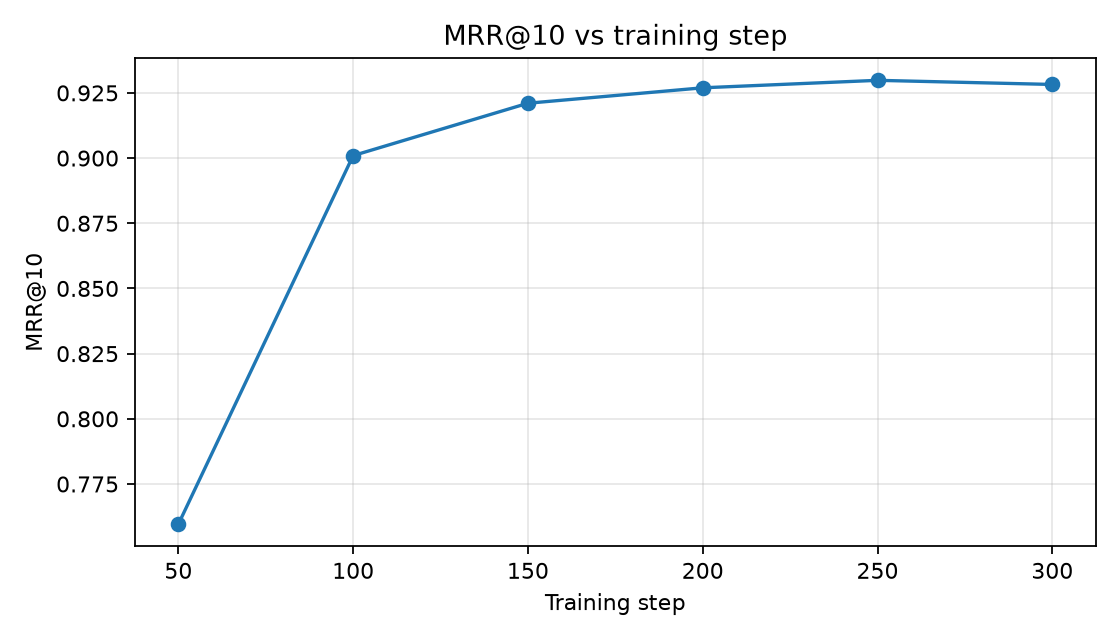
\includegraphics[width=\linewidth]{assets/plots/MRRat10.png}
\end{subfigure}
\begin{subfigure}{0.31\textwidth}
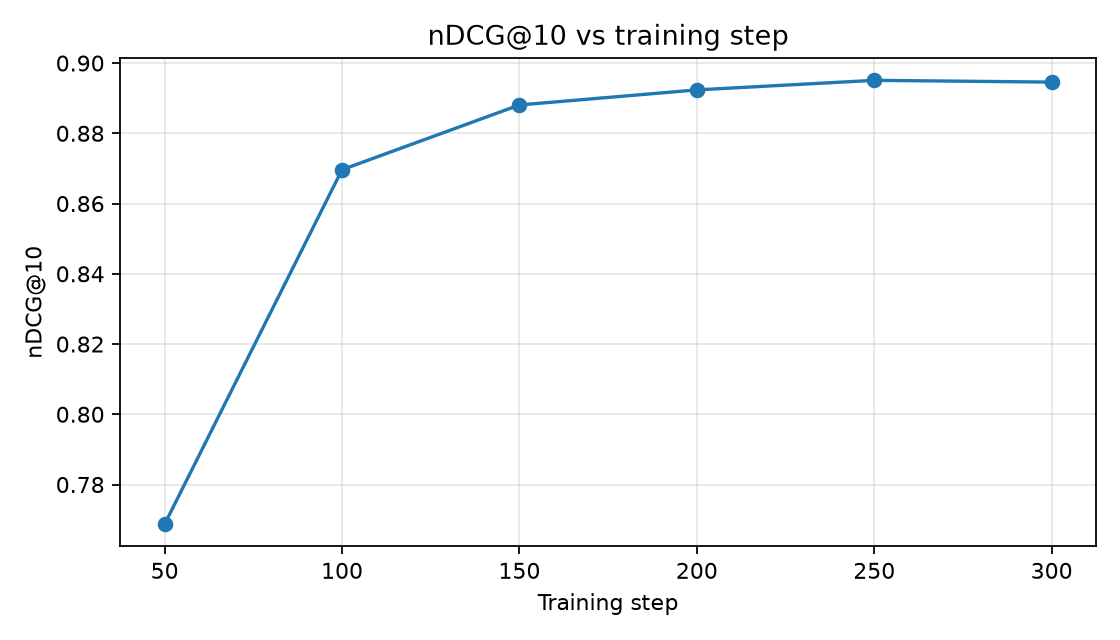
\includegraphics[width=\linewidth]{assets/plots/nDCGat10.png}
\end{subfigure}
\begin{subfigure}{0.31\textwidth}
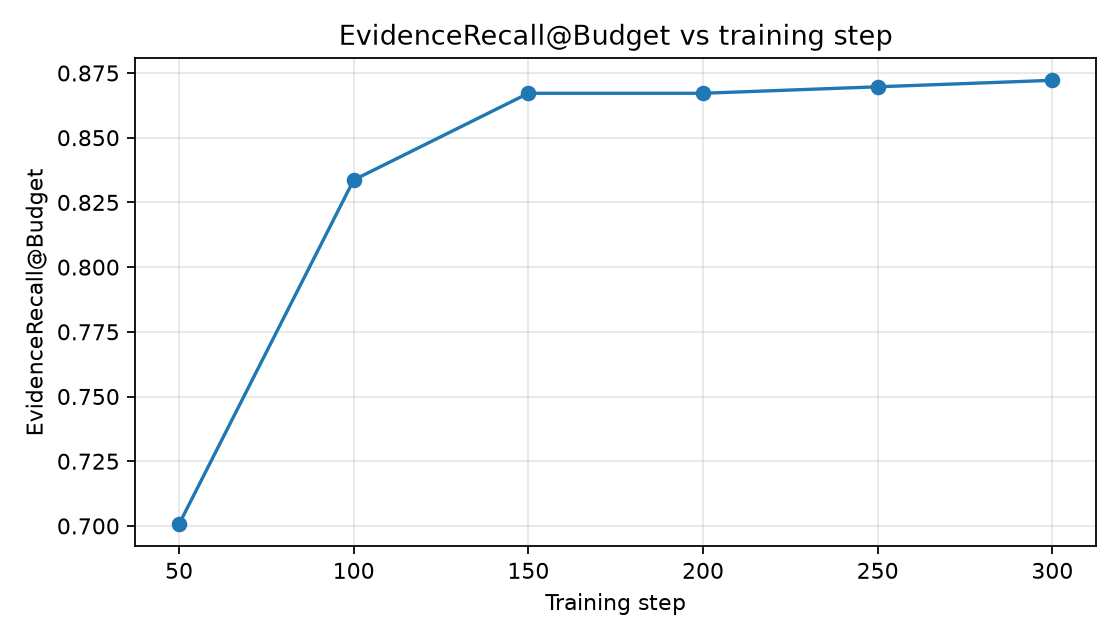
\includegraphics[width=\linewidth]{assets/plots/EvidenceRecallatBudget.png}
\end{subfigure}

\begin{subfigure}{0.31\textwidth}
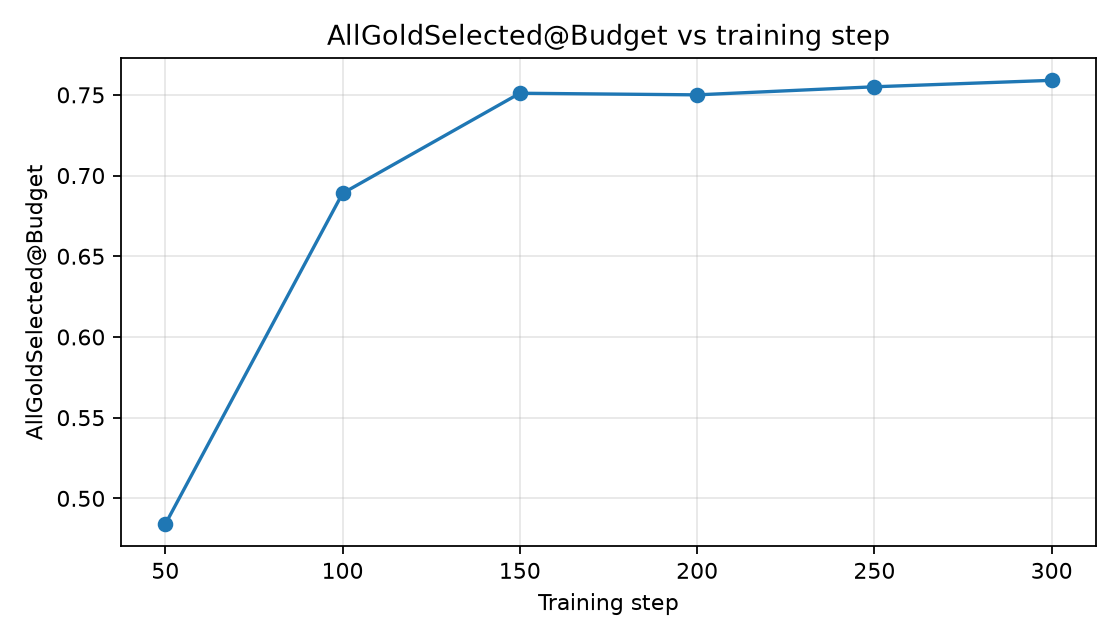
\includegraphics[width=\linewidth]{assets/plots/AllGoldSelectedatBudget.png}
\end{subfigure}
\begin{subfigure}{0.31\textwidth}
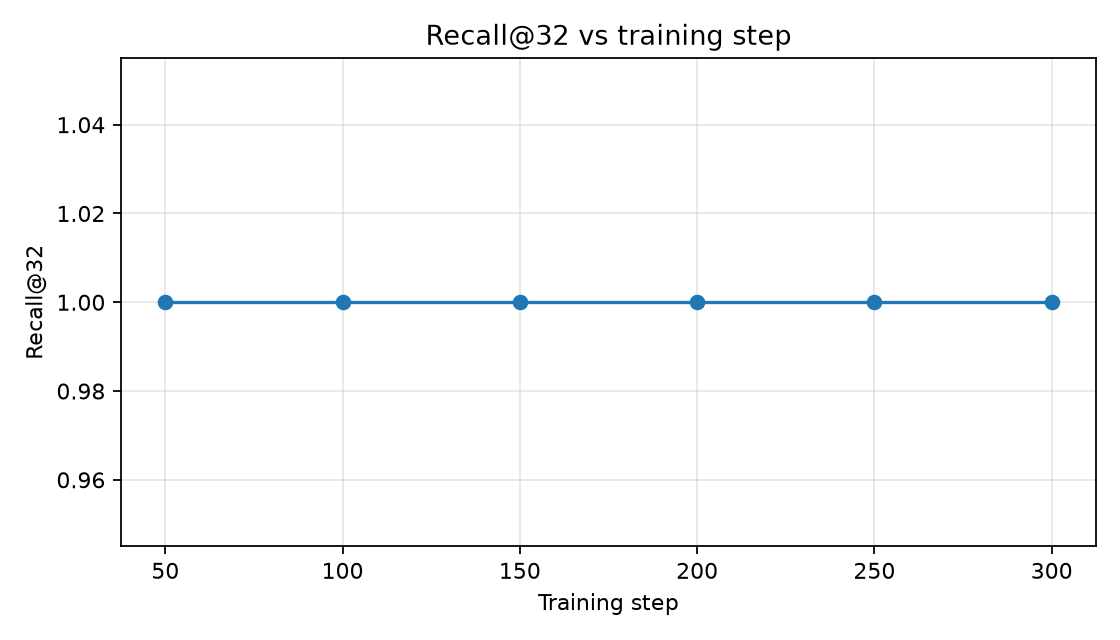
\includegraphics[width=\linewidth]{assets/plots/Recallat32.png}
\end{subfigure}
\begin{subfigure}{0.31\textwidth}
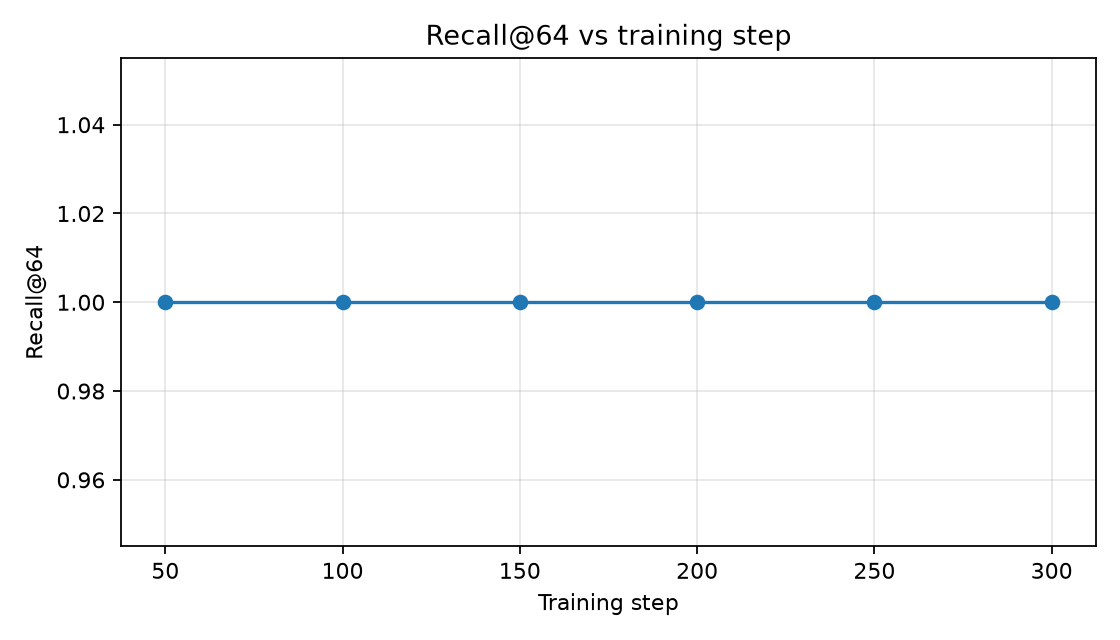
\includegraphics[width=\linewidth]{assets/plots/Recallat64.png}
\end{subfigure}

\begin{subfigure}{0.31\textwidth}
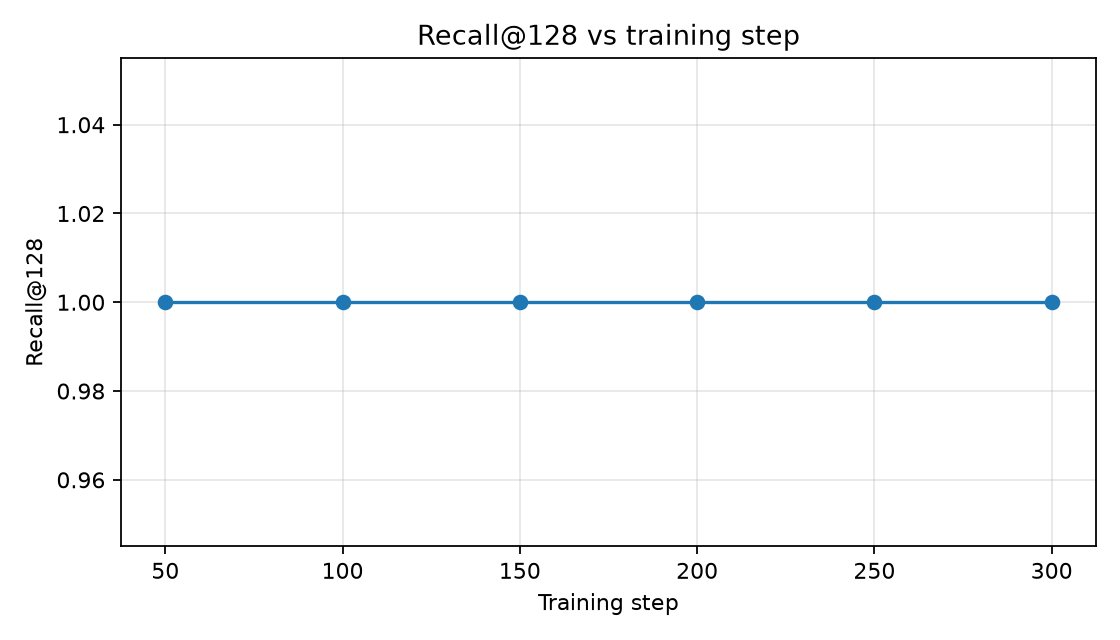
\includegraphics[width=\linewidth]{assets/plots/Recallat128.png}
\end{subfigure}
\begin{subfigure}{0.31\textwidth}
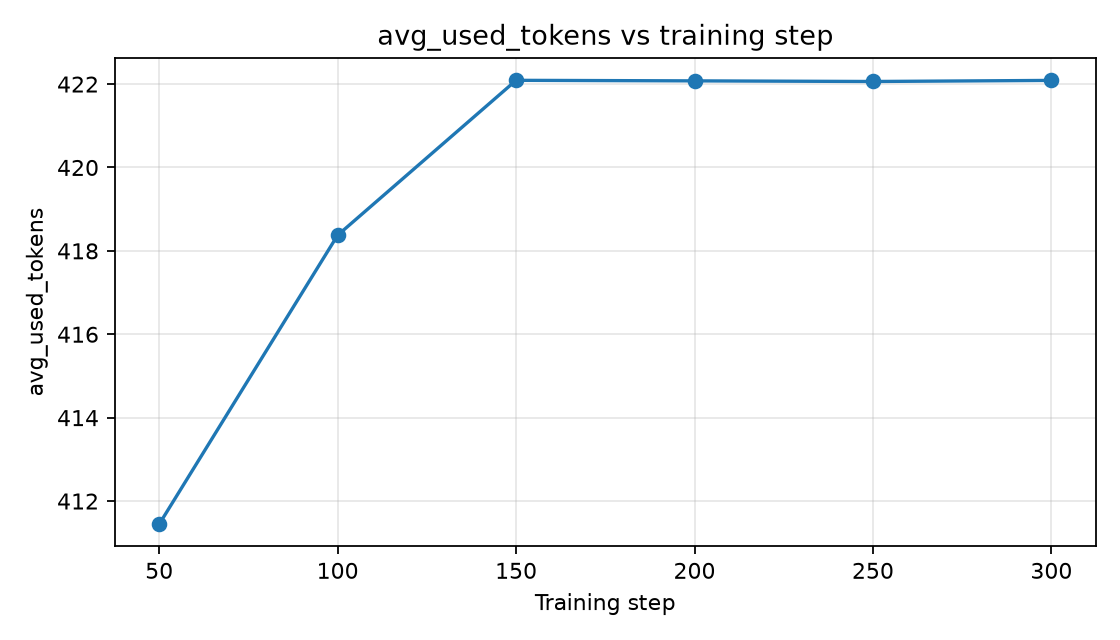
\includegraphics[width=\linewidth]{assets/plots/avg_used_tokens.png}
\end{subfigure}
\begin{subfigure}{0.31\textwidth}
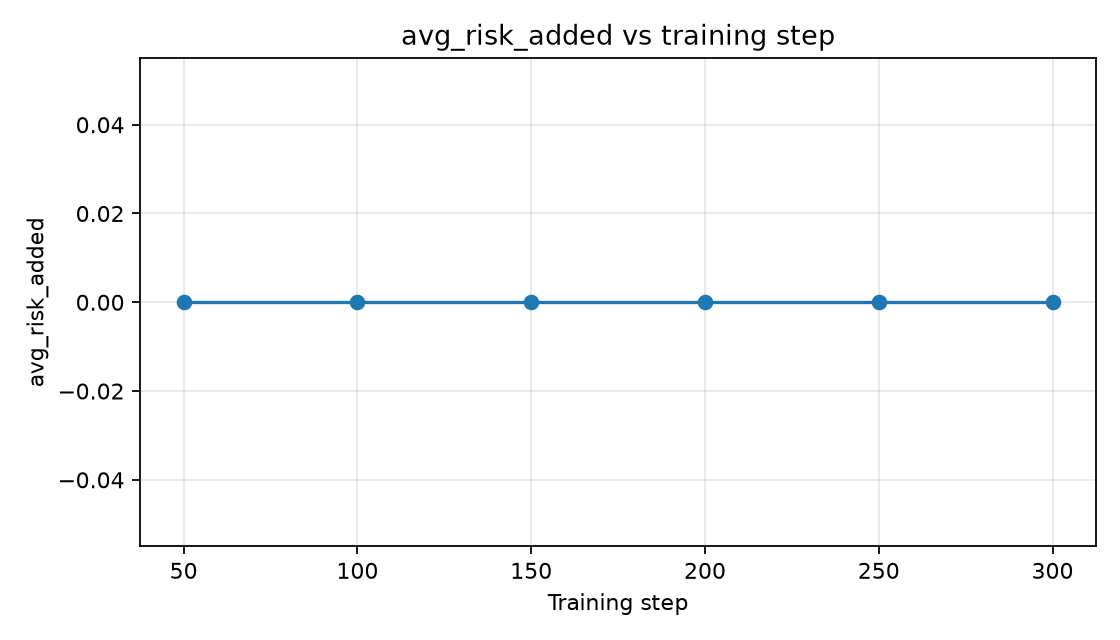
\includegraphics[width=\linewidth]{assets/plots/avg_risk_added.png}
\end{subfigure}
\caption{Metric curves across the six saved checkpoints.}
\end{figure*}

\section{Conclusion}
EvidenceCodec reached a useful working baseline within the time limit. The system built full HotpotQA artifacts, trained ModernBERT-large checkpoints, evaluated every checkpoint, and produced metric curves. The final checkpoint preserved 87.2 percent of annotated evidence under budget and selected all annotated gold evidence for 75.9 percent of validation examples. For a short run, this is a strong result and a good foundation for longer training and broader evaluation.

\end{document}
